
%!TEX TS-program = xelatex
\documentclass[]{friggeri-cv}
\usepackage{afterpage}
\usepackage{hyperref}
\usepackage{color}
\usepackage{xcolor}
\usepackage{smartdiagram}
\usepackage{fontspec}
% if you want to add fontawesome package
% you need to compile the tex file with LuaLaTeX
% References:
%   http://texdoc.net/texmf-dist/doc/latex/fontawesome/fontawesome.pdf
%   https://www.ctan.org/tex-archive/fonts/fontawesome?lang=en
%\usepackage{fontawesome}
\usepackage{metalogo}
\usepackage{dtklogos}
\usepackage[utf8]{inputenc}
\usepackage{tikz}
\usepackage{multicol}
\usepackage{setspace}
\usepackage[document]{ragged2e}
%\usepackage{titlesec}
%\usepackage[skip=4pt, indent=0.0pt, parfill=4.0pt]{parskip}
\usetikzlibrary{mindmap,shadows}
\hypersetup{
    pdftitle={},
    pdfauthor={},
    pdfsubject={},
    pdfkeywords={},
    colorlinks=false,           % no lik border color
    allbordercolors=white       % white border color for all
}
\smartdiagramset{
    bubble center node font = \footnotesize,
    bubble node font = \footnotesize,
    % specifies the minimum size of the bubble center node
    bubble center node size = 0.5cm,
    %  specifies the minimum size of the bubbles
    bubble node size = 0.5cm,
    % specifies which is the distance among the bubble center node and the other bubbles
    distance center/other bubbles = 0.3cm,
    % sets the distance from the text to the border of the bubble center node
    distance text center bubble = 0.5cm,
    % set center bubble color
    bubble center node color = pblue,
    % define the list of colors usable in the diagram
    set color list = {lightgray, materialcyan, orange, green, materialorange, materialteal, materialamber, materialindigo, materialgreen, materiallime},
    % sets the opacity at which the bubbles are shown
    bubble fill opacity = 0.6,
    % sets the opacity at which the bubble text is shown
    bubble text opacity = 0.5,
}

\addbibresource{bibliography.bib}
\RequirePackage{xcolor}
\definecolor{pblue}{HTML}{0395DE}

%\titlespacing*{\section}
%{0pt}{12pt plus 4pt minus 2pt}{0pt plus 2pt minus 2pt}
%\titlespacing*{\subsection}
%{0pt}{12pt plus 4pt minus 2pt}{0pt plus 2pt minus 2pt}
%\titlespacing*{\subsubsection}
%{0pt}{12pt plus 4pt minus 2pt}{0pt plus 2pt minus 2pt}

\title{Yoann Chamillard -- Resume}
\author{Yoann Chamillard}
\date{07/6/2025}

\hypersetup{
  pdftitle={Yoann Chamillard -- Resume},
  pdfauthor={Yoann Chamillard},
  pdfsubject={Ingénieur Développeur Web \& Mobile Full Stack - Resume},
  pdfkeywords={profile:webDev; resume; developer; software; engineer; C\# .Net; Python; Javascript; Node.js; Java; Kotlin; Android; Rest API; Git  GitLab; Docker; Jenkins; Selenium; Cron; Html-Css; MySQL; PostgreSQL; MongoDB; SQLite; Firebase; Bash; Jira; Regex; createdAt:2025-06-07 10:56:45.731598 ; id:d527a0},
  pdfcreator={LuaLaTeX},
  pdfproducer={LuaLaTeX}
}

\begin{document}

\header{Yoann}{Chamillard}
      {~~~~~~~~~~~~~~~~Ingénieur Développeur Web Full Stack}
      {}

\begin{aside}
\hspace{10mm}
\includegraphics[scale=0.148]{Photo_CV.jpg}
\section{Infos}

%33 ans\\
Permis A,B\\
\vspace{2.5mm}
Paris, France\\
\vspace{1.5mm}
Mobile à l'international\\
Autorisé à travailler au Canada (visa PVT)\\
\vspace{2.5mm}
+33 670525552\\
\href{mailto:yoann.chamillard@gmail.com}{\small yoann.chamillard@gmail.com}\\
\vspace{2.5mm}
\href{http://fr.linkedin.com/in/yoannchamillard}{LinkedIn\hspace{1.5mm}
\includegraphics[scale=0.075]{hlink.png}}\\
\href{https://github.com/Nokheenig?tab=stars}{GitHub\hspace{1.5mm}
\includegraphics[scale=0.075]{hlink.png}}\\
\vspace{2.5mm}
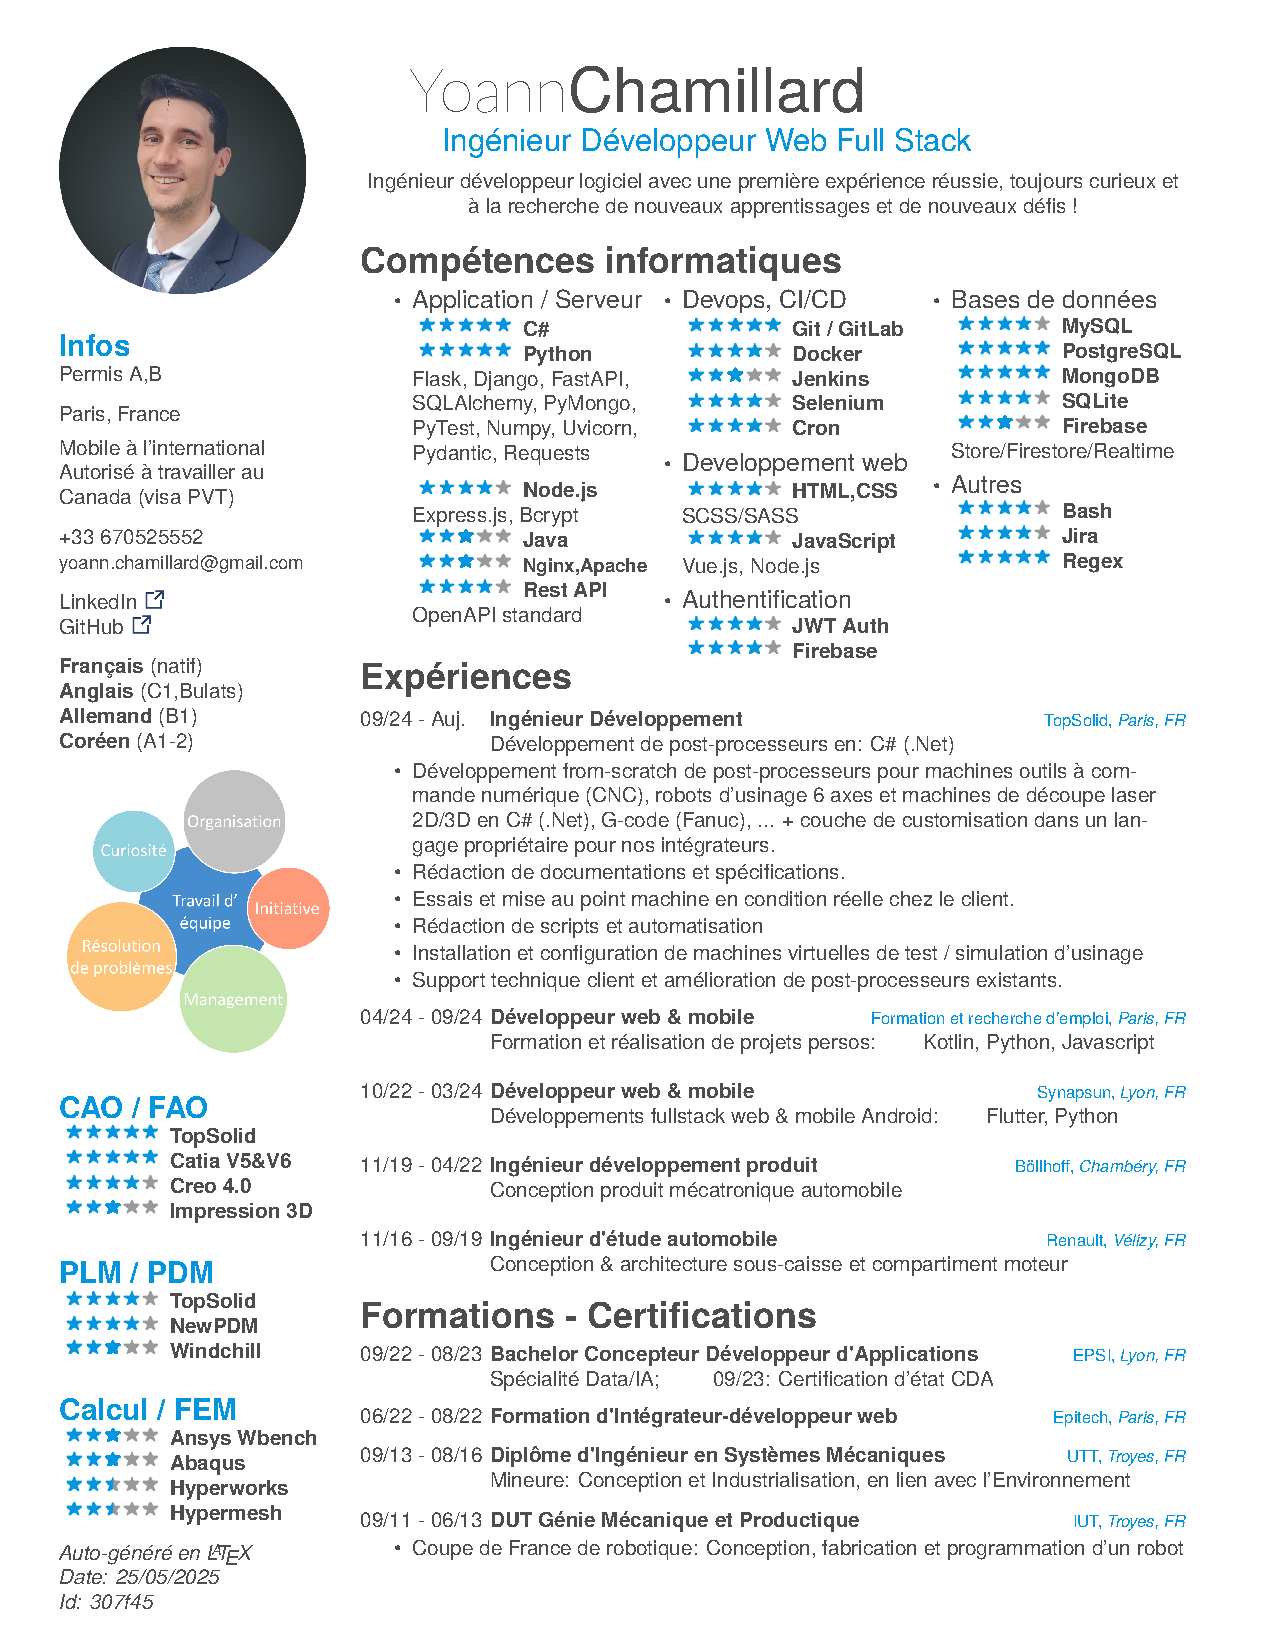
\includegraphics[width=1.5cm,height=3cm,keepaspectratio]{qr/resume_FR_webDev.png}\\
\vspace{2.5mm}
\makebox[4.3cm][l]{\textbf{Français} (natif)}\\
\makebox[4.3cm][l]{\textbf{Anglais} (C1,Bulats)}\\
\makebox[4.3cm][l]{\textbf{Allemand} (B1)}\\
\makebox[4.3cm][l]{\textbf{Coréen} (A1-2)}\\
\vspace{2.5mm}%

\section{Points forts}
\begin{itemize}
\item Travail d'équipe
\item Curiosité/Créativité
\item Initiative
\item Organisation
\item Adaptabilité
\end{itemize}
\section{Mécanique}
\begin{itemize}
\item CAO
 \\ \hspace*{0.2em}\small\textit{Catia, Creo, TopSolid}
\item FAO
 \\ \hspace*{0.2em}\small\textit{TopSolid}
\item PDM
 \\ \hspace*{0.2em}\small\textit{NewPDM, Windchill, TopSolid}
\item Calcul/FEM
 \\ \hspace*{0.2em}\small\textit{Ansys, Abaqus, Hyperworks}
\item Impression 3D
\end{itemize}
\section{Centres d'intérêt}
\begin{itemize}
\item Randonnée
\item Musique / Concerts
\item Moto / Vélo
\item Photographie
\item Voyages
\end{itemize}
\vspace{2.5mm}%\begin{flushleft}
\small \emph{Auto-généré en \LaTeX}\\
\small \emph{Date: 07/06/2025} \hspace*{8mm}\\
\small \emph{Id: d527a0} % resumeId\\
%{\tiny d527a0}\\ % resumeId

	%\end{flushleft}
\end{aside}

\vspace*{-2.0mm}
\noindent\parbox{\linewidth}{
  \centering
  Ingénieur développeur logiciel avec une première expérience réussie, toujours curieux et à la recherche de nouveaux apprentissages et de nouveaux défis !
}
\vspace*{0.8mm}

\section{Compétences informatiques}
        \vspace*{-0.45cm}
        \setlength{\columnsep}{-0.3cm}
        \begin{flushleft}
        \begin{multicols}{3}
		\begin{itemize}
		
		\setlength{\itemsep}{5pt}
  		\setlength{\parskip}{0pt}
  		\setlength{\parsep}{0pt}
          
        
\item \large Application / Serveur \
\normalsize
\begin{flushleft}


\includegraphics[scale=0.40]{5stars.png}\hspace{1.5mm}\textbf{C\#}

\includegraphics[scale=0.40]{5stars.png}\hspace{1.5mm}\textbf{Python}\\Flask, Django, FastAPI, SQLAlchemy, PyMongo, PyTest, Numpy, Uvicorn, Pydantic, Requests\\\vspace{2mm}

\includegraphics[scale=0.40]{4stars.png}\hspace{1.5mm}\textbf{Node.js}\\Express.js, Bcrypt\\

\includegraphics[scale=0.40]{3stars.png}\hspace{1.5mm}\textbf{Java}

\includegraphics[scale=0.40]{3stars.png}\hspace{1.5mm}\textbf{\small Nginx,Apache}

\includegraphics[scale=0.40]{4stars.png}\hspace{1.5mm}\textbf{Rest API}\\OpenAPI standard\\
\end{flushleft}            

\columnbreak
\item \large Devops, CI/CD \
\normalsize
\begin{flushleft}


\includegraphics[scale=0.40]{5stars.png}\hspace{1.5mm}\textbf{Git / GitLab}

\includegraphics[scale=0.40]{4stars.png}\hspace{1.5mm}\textbf{Docker}

\includegraphics[scale=0.40]{3stars.png}\hspace{1.5mm}\textbf{Jenkins}

\includegraphics[scale=0.40]{4stars.png}\hspace{1.5mm}\textbf{Selenium}

\includegraphics[scale=0.40]{4stars.png}\hspace{1.5mm}\textbf{Cron}
\end{flushleft}            

\item \large Developpement web \
\normalsize
\begin{flushleft}


\includegraphics[scale=0.40]{4stars.png}\hspace{1.5mm}\textbf{HTML,CSS}\\SCSS/SASS\\

\includegraphics[scale=0.40]{4stars.png}\hspace{1.5mm}\textbf{JavaScript}\\Vue.js, Node.js\\
\end{flushleft}            

\item \large Authentification \
\normalsize
\begin{flushleft}


\includegraphics[scale=0.40]{4stars.png}\hspace{1.5mm}\textbf{JWT Auth}

\includegraphics[scale=0.40]{4stars.png}\hspace{1.5mm}\textbf{Firebase}
\end{flushleft}            

\columnbreak
\item \large Bases de données \
\normalsize
\begin{flushleft}


\includegraphics[scale=0.40]{4stars.png}\hspace{1.5mm}\textbf{MySQL}

\includegraphics[scale=0.40]{5stars.png}\hspace{1.5mm}\textbf{PostgreSQL}

\includegraphics[scale=0.40]{5stars.png}\hspace{1.5mm}\textbf{MongoDB}

\includegraphics[scale=0.40]{4stars.png}\hspace{1.5mm}\textbf{SQLite}

\includegraphics[scale=0.40]{3stars.png}\hspace{1.5mm}\textbf{Firebase}\\Store/Firestore/Realtime\\
\end{flushleft}            

\item \large Autres \
\normalsize
\begin{flushleft}


\includegraphics[scale=0.40]{4stars.png}\hspace{1.5mm}\textbf{Bash}

\includegraphics[scale=0.40]{4stars.png}\hspace{1.5mm}\textbf{Jira}

\includegraphics[scale=0.40]{5stars.png}\hspace{1.5mm}\textbf{Regex}

\includegraphics[scale=0.40]{5stars.png}\hspace{1.5mm}\textbf{Office}
\end{flushleft}            


        \end{itemize}
        \end{multicols}
        %\end{itemize}
        \end{flushleft} \normalsize
        \vspace*{-0.65cm}
\section{Expériences}
\vspace*{-0.25cm}

\begin{entrylist}
  \entry
    {09/24 - Auj.}
    {Ingénieur Développement}
    {TopSolid, \textit{Paris, FR}}
    {Développement de post-processeurs en:  C\# (.Net)}
\end{entrylist}
\vspace{-15pt}

\vspace{0.5mm}
\begin{itemize}
\setlength{\itemsep}{1pt}
\setlength{\parskip}{0pt}
\setlength{\parsep}{0pt}

\item Développement from-scratch de post-processeurs pour machines outils à commande numérique (CNC), robots d'usinage 6 axes et machines de découpe laser 2D/3D en C\# (.Net), G-code (Fanuc), ... + couche de customisation dans un langage propriétaire pour nos intégrateurs.
\item Rédaction de documentations et spécifications.
\item Essais et mise au point machine en condition réelle chez le client.
\item Rédaction de scripts et automatisation
\item Installation et configuration de machines virtuelles de test / simulation d'usinage
\item Support technique client et amélioration de post-processeurs existants.
\end{itemize}

\begin{entrylist}
  \entry
    {04/24 - 09/24}
    {Développeur web \& mobile}
    {Formation et recherche d'emploi, \textit{Paris, FR}}
    {Formation et réalisation de projets persos:\hspace*{8mm}Kotlin, Python, Javascript}
\end{entrylist}

\begin{entrylist}
  \entry
    {10/22 - 03/24}
    {Développeur web \& mobile}
    {Synapsun, \textit{Lyon, FR}}
    {Développements fullstack web \& mobile Android:\hspace*{8mm}Flutter, Python}
\end{entrylist}

\begin{entrylist}
  \entry
    {11/19 - 04/22}
    {Ingénieur développement produit}
    {Böllhoff, \textit{Chambéry, FR}}
    {Conception produit mécatronique automobile}
\end{entrylist}

\begin{entrylist}
  \entry
    {11/16 - 09/19}
    {Ingénieur d'étude automobile}
    {Renault, \textit{Vélizy, FR}}
    {Conception \& architecture sous-caisse et compartiment moteur}
\end{entrylist}

\vspace*{-0.5cm}
\vspace*{0.45cm}
\section{Formations - Certifications}
\vspace*{-0.25cm}
\vspace{0.5mm}
    \begin{entrylist}
    \entry
        {09/22 - 08/23}
        {Bachelor Concepteur Développeur d'Applications}
        {EPSI, \textit{Lyon, FR}}
        {Spécialité Data/IA; \hspace{7mm} 09/23: Certification d'état CDA}
    \end{entrylist}
    \vspace{0.5mm}
\begin{entrylist}
\entry
    {06/22 - 08/22}
    {Formation d'Intégrateur-développeur web}
    {Epitech, \textit{Paris, FR}}
    {}
\end{entrylist}
\vspace{0.5mm}
    \begin{entrylist}
    \entry
        {09/13 - 08/16}
        {Diplôme d'Ingénieur en Systèmes Mécaniques}
        {UTT, \textit{Troyes, FR}}
        {Mineure: Conception et Industrialisation, en lien avec l’Environnement}
    \end{entrylist}
    \vspace{0.5mm}
\begin{entrylist}
\entry
    {09/11 - 06/13}
    {DUT Génie Mécanique et Productique}
    {IUT, \textit{Troyes, FR}}
    {}
\end{entrylist}
\vspace*{-0.7cm}
\begin{itemize}
\setlength{\itemsep}{1pt}
\setlength{\parskip}{0pt}
\setlength{\parsep}{0pt}
\item Coupe de France de robotique: Conception, fabrication et programmation d’un robot
\end{itemize}
\end{document}